\documentclass{article}
\usepackage{lipsum} % For placeholder text, remove in final document
\usepackage{float} % For better figure placement
\usepackage{hyperref}
\usepackage{graphicx} % Required for inserting images

\title{Machine Learning Evaluation Report}
\author{NAMUGGA MARTHA  -21/U/0863 \\ 
AGABA TRISHA ESTHER  -21/U/1055 \\ 
ARIHO CONRAD  -21/U/05873/PS \\
MUMBERE ASINGYA JOSHUA  -21/U/13667/EVE \\
BIRIMUMAASO ROGERS T  -21/U/11851/PS}

\date{\today}

\begin{document}

\maketitle

\section{Introduction}
In this report, we present an evaluation of various machine learning models applied to predict math scores based on reading and writing scores. The models include Random Forest, Gradient Boosting, Support Vector Machine (SVM), and a Neural Network. The objective is to assess the performance of these models in predicting math scores using different algorithms and approaches.

\section{Dataset}
The dataset used in this analysis consists of student performance data, including reading scores, writing scores, and math scores. The features are used to predict the math scores of students.

\section{Methodology and Algorithm Architecture}
We employed several machine learning algorithms to build predictive models for math scores:
\begin{itemize}
\item Random Forest
\item Gradient Boosting
\item Support Vector Machine (SVM)
\item Neural Network
\end{itemize}

The Random Forest and Gradient Boosting models are part of the sklearn library, while the Support Vector Machine is implemented using the SVR module. The Neural Network is developed using TensorFlow and Keras.

\begin{figure}[H]
\centering
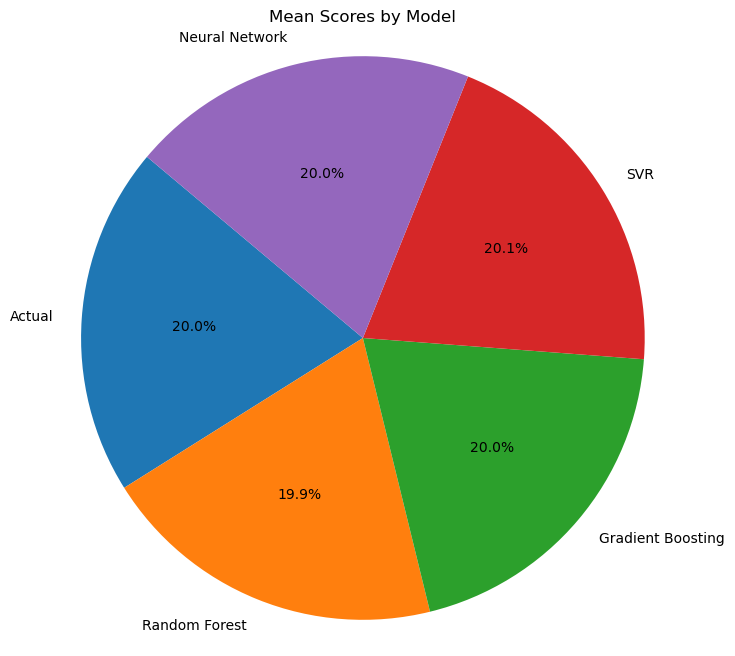
\includegraphics[width=0.8\textwidth]{algorithm_architecture.png}
\caption{Mean Scores by each Model}
\label{fig:algorithm_architecture}
\end{figure}

Figure \ref{fig:algorithm_architecture} illustrates  the  Mean Scores by each Model used in this analysis.

\section{Evaluation Metrics}
We evaluated the performance of each model using Mean Absolute Error (MAE), a metric that measures the average magnitude of errors between actual and predicted values.

\section{Results and Results Discussion}
The results of the evaluation are as follows:
\begin{itemize}
\item Random Forest MAE: 7.884305662962641
\item Gradient Boosting MAE: 7.251805446162537
\item SVM MAE: 7.073221628608613
\item Neural Network MAE: 7.007719596862793
\end{itemize}

From the results, we observed that the Neural Network model achieved the lowest MAE, indicating better performance in predicting math scores compared to other models.

\section{Limitations of the Work}
One limitation of our analysis is the limited size of the dataset, which may impact the generalizability of the models. Additionally, the choice of hyperparameters and model complexity could influence the results.

\section{Conclusion and Future Work}
In conclusion, our evaluation demonstrates the effectiveness of machine learning models, particularly the Neural Network, in predicting math scores based on reading and writing scores. For future work, we plan to explore larger datasets and fine-tune model parameters to improve predictive accuracy.

\end{document}
